\chapter{Quantum repeaters}
\label{sec:12_quantum_repeaters}
\label{ch:repeaters}

\section{The need for repeaters}
\label{sec:12-1_need_for_repeaters}

In the previous Chapter, we have seen that there is one big problem when trying to communicate over long distances, and that's photon loss in fibers.
The farther we are trying to communicate, the more likely we are to lose the photon.
There's also another problem, and that's the number of devices that are connected to the network. Currently (2022) there are 8 billion people, and an estimated 31 billion Internet of Things devices.
Despite this staggering number, all of these devices can communicate with each other.
How is this achieved?
One way is to establish a direct connection between each device that is present in the network as shown in the left panel of Fig.~\ref{fig:12-1_all_to_all}.
Two devices are connected by a single link.
Three devices require three links, four devices require six links and so on.
For $N$ devices, $N (N - 1) / 2$ links are needed in order to have all-to-all coupling.

\begin{figure}[t]
    \centering
    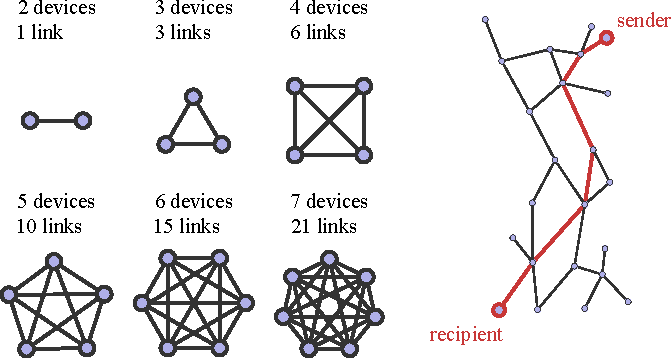
\includegraphics[width=0.85\textwidth]{lesson12/12-1_all_to_all.pdf}
    \caption[All-to-all coupling]{Right panel shows how many links are required to have all-to-all coupling. Left panel shows a more realistic network topology and the path along which a qubit needs to be teleported from sender to a receiver.}
    \label{fig:12-1_all_to_all}
\end{figure}

Real networks do not use all-to-all coupling.
Each individual link requires dedicated hardware that is allowing communication between two devices in the network.
Adding a single device to the network would also require to add links to all existing devices.
Such an approach is clearly not practical even for relatively small networks.
The right panel of Fig.~\ref{fig:12-1_all_to_all} shows a much more realistic network, where an arbitrary sender can still transmit a message to the intended receiver, even in the absence of a direct link between the two.

In quantum networks, information encoded in qubits is not transmitted directly.
Rather we use entangled pairs to teleport the state of the qubit as discussed in Chapter~\ref{sec:8_teleportation}.
Each link connecting two devices shares a Bell pair which is used to pass the state of the qubit carrying the quantum message from one device to the next.
We can go back to the right panel of Fig.~\ref{fig:12-1_all_to_all} and this time think of as a quantum network, where the quantum sender wishes to pass the state of a qubit to the recipient.
The state of the sender's qubit can be teleported hop-by-hop along the red path until it reaches the recipient.
A problem with this approach is that the operations required by the teleportation protocol as well as the memories used to store Bell pairs are not perfect.
This in turn decreases the fidelity of the teleported qubit.
Repeating the teleportation in this hop-by-hop approach deteriorates the fidelity further resulting in a completely garbled quantum state being teleported to the recipient.
A way around this problem is to use the link-level Bell pairs to create a direct entangled connection between the sender and the recipient so that the quantum state can be teleported in one hop.
The quantum nodes that achieving this splicing of link-level entanglement are called \textit{\textbf{quantum repeaters}}, and they are indispensable in the design of long-distance quantum networks.

We will address four requirements in this chapter.
First, we will show how to establish entanglement between neighboring nodes of a quantum network. This is known link-level entanglement.
Next, we will discuss how the link-level entanglement can be used to create a long-distance entangled connection between end nodes using entanglement swapping.
After this, we will deal with the issues presented by the adverse effects of noise.
Finally, we will look at management of networks, routing, multiplexing and resource management.


\section{Making link-level entanglement}
\label{sec:12-2_making_link_level_rantanglement}

In this section, we consider the task of creating link-level entanglement between two neighboring repeaters of a quantum network.
One way of entangling two quantum memories and creating link-level entanglement is pictured in Fig.~\ref{fig:12-2_MIM}, and is known as \textit{\textbf{memory-interfere-memory}} (MIM) link architecture.
Other names for this architecture are memory-interfere-memory or meet-in-the-middle.
Each repeater node is equipped with a quantum memory, and is coupled to an optical fiber.
The fibers lead to a \textit{\textbf{Bell state analyzer}} (BSA), an optical device which is capable of measuring incoming photons in the Bell basis.
We will discuss an implementation of the BSA in Section~\ref{sec:13-3_Bell_state_measurement_2}.

\begin{figure}[t]
    \centering
    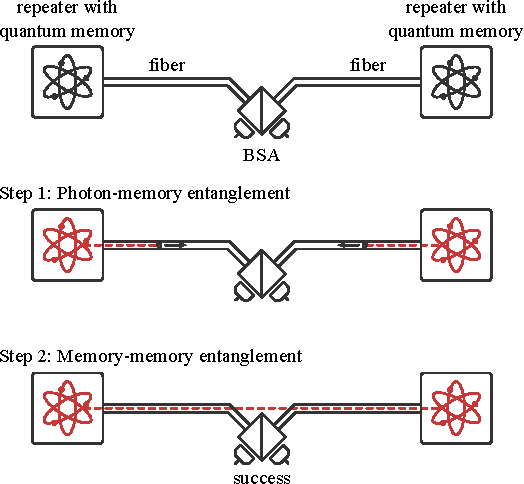
\includegraphics[width=0.8\textwidth]{lesson12/12-2_MIM.pdf}
    \caption[MIM link architecture]{MIM link architecture.}
    \label{fig:12-2_MIM}
\end{figure}

The protocol to generate entanglement between the quantum memories is the following.
The quantum memories are made to emit a photon which is entangled with the memory, represented by the red dashed line in Fig.~\ref{fig:12-2_MIM}.
These photons are captured and coupled to a fiber which guides them to the BSA.
At the BSA they are measured in the Bell basis and destroyed in the process.
The success probability of the Bell state measurement depends on the implementation of the BSA.
For BSA implemented using linear optics elements, which is one of the more straightforward implementations, the success probability is at most $50\%$.
This is a assuming ideal couplers (to collect photons emitted by the memories), fibers, and detectors at the BSA.
Once the measurement is successful, the entanglement between the memory-photon pairs is transferred to be between the memories and the link-level entanglement is established.

Crucial point about this scheme, and other link-level architectures, is that the photons arriving at the BSA to be measured in the Bell basis must be \textit{\textbf{indistinguishable}}.
This can be achieved by arranging that the photons arrive simultaneously. 
Even relatively small delays in their arrival times reduce the indistinguishability of the photons resulting in a vanishing success probability of the Bell state measurement.

\begin{figure}[t]
    \centering
    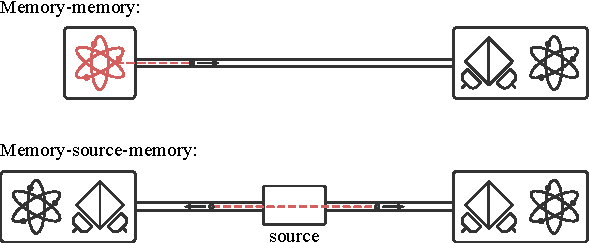
\includegraphics[width=0.85\textwidth]{lesson12/12-2_MM_MSM.pdf}
    \caption[MM and MSM architectures]{Memory-memory and Memory-source-memory link-level architectures.}
    \label{fig:12-2_MM_MSM}
\end{figure}

Figure~\ref{fig:12-2_MM_MSM} shows two more link-level architectures.
The first one is \textit{\textbf{memory-memory}} (MM), where the BSA device is included in one the repeater nodes.
Entanglement is established in a similar way as for the MIM architecture, but this time photon generated by the quantum memory on the left travels the whole length of the fiber to the right node.
There it interferes with a photon emitted by the right quantum memory.
This architecture sometimes called the sender-receiver architecture.
The bottom panel of Fig.~\ref{fig:12-2_MM_MSM} shows the \textit{\textbf{memory-source-architecture}} (MSM) architecture.
This time, a source of entangled photon pairs located between the quantum repeaters is used.
These photons are sent to the quantum repeaters where they interfere with photons emitted locally by the quantum memories.


\section{Reaching for distance: Entanglement swapping}
\label{sec:fig:12-3_reaching_for_distance}

In the previous step, we have seen how to establish link-level entanglement.
We will now extend it to establishing long-distance entanglement spanning multiple hops.
Consider three network nodes represented by Repeater 0, Repeater 1 is holding two qubits, and Repeater 2.
We assume that link-level entanglement has been established between Repeater 0 and one of the qubits at Repeater 1, and the other qubit at Repeater 1 and Repeater 2.
The goal is to establish entanglement between Repeater 0 and Repeater 2.

\begin{figure}[t]
    \centering
    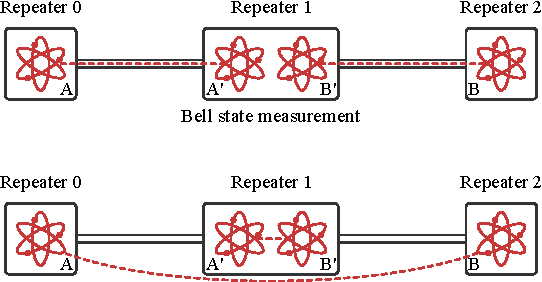
\includegraphics[width=0.8\textwidth]{lesson12/12-3_entanglement_swapping.pdf}
    \caption[Entanglement swapping]{Entanglement swapping at Repeater 1 creates entanglement between Repeaters 0 and 2.}
    \label{fig:12-3_entanglement_swapping}
\end{figure}

This is achieved by measuring the two qubits at Repeater 1 in the Bell basis.
This measurement projects them onto one of the four Bell pairs.
At the same the effect of this measurement is to also project the qubits at Repeater 0 and Repeater 2 onto a Bell pair, effectively creating entanglement between these two repeaters.
This procedure is known as \textit{\textbf{entanglement swapping}}, and it is an indispensable tool in creating long-distance entanglement in quantum networks.
Note that this entanglement is between two repeaters which are not directly connected.

Let's now get a little technical and show that Repeater 0 and Repeater 2 are entanglement more rigorously.
We label the qubit at Repeater 0 by $A$ and the qubit that is entangled with it at Repeater 1 is labelled by $A^{\prime}$.
The other qubit at Repeater 1 is denoted by $B^{\prime}$, and its entangled partner at Repeater 2 by $B$.
The state of the qubits is one of the Bell pairs, let's say $|\Phi^+\rangle$.
Same goes for the pair of qubits $BB^{\prime}$.
The total state of the four qubits can therefore be written as
\begin{align}
    \begin{aligned}
        \ket{\psi} & = \ket{\Phi^{+}}_{A A^{\prime}}\ket{\Phi^{+}}_{B^{\prime} B} \\
        & = \frac{1}{2} ( |0000\rangle+|0011\rangle+|1100\rangle+|1111\rangle ).
        \label{eq:12-3_computational_basis}
    \end{aligned}
\end{align}

In the next step of our calculation, we will use a little trick.
We rewrite the state of the qubits at Repeater 1, $A^{\prime}B^{\prime}$ as superpositions of the Bell states,
\begin{align}
|00\rangle & = \left(\left|\Phi^{+}\right\rangle+\left|\Phi^{-}\right\rangle\right) / \sqrt{2}, \\
|01\rangle & = \left(\left|\Psi^{+}\right\rangle+\left|\Psi^{-}\right\rangle\right) / \sqrt{2}, \\
|10\rangle & = \left(\left|\Psi^{+}\right\rangle-\left|\Psi^{-}\right\rangle\right) / \sqrt{2}, \\
|11\rangle & = \left(\left|\Phi^{+}\right\rangle-\left|\Phi^{-}\right\rangle\right) / \sqrt{2}.
\end{align}
We can now use these identities in Eq.~(\ref{eq:12-3_computational_basis}) and rewrite the total state of the four qubits as follows,
\begin{align}
    |\psi\rangle_{AA^{\prime}B^{\prime}B} & = \frac{1}{2\sqrt{2}} \left[ |0\rangle (|\Phi^+\rangle + |\Phi^-\rangle) |0\rangle + |0\rangle (|\Psi^+\rangle + |\Psi^-\rangle) |1\rangle \right. \nonumber\\
    & + \left. |1\rangle (|\Psi^+\rangle - |\Psi^-\rangle) |0\rangle + |1\rangle (|\Phi^+\rangle - |\Phi^-\rangle) |1\rangle \right].
\end{align}
We can group the qubits that are going to be measured on the left, and the qubits that we are not going to measure on the right,
\begin{align}
    |\psi\rangle_{A^{\prime}B^{\prime}AB} & = \frac{1}{2\sqrt{2}} \left[ (|\Phi^+\rangle + |\Phi^-\rangle)|0\rangle|0\rangle + (|\Psi^+\rangle + |\Psi^-\rangle)|0\rangle|1\rangle \right. \nonumber\\
    & + \left. (|\Psi^+\rangle - |\Psi^-\rangle)|1\rangle|0\rangle + (|\Phi^+\rangle - |\Phi^-\rangle)|1\rangle|1\rangle \right].
\end{align}
We have not really done anything apart from rearranging the qubits.
Finally, we group the terms according to which Bell state they are in,
\begin{align}
    |\psi\rangle_{A^{\prime}B^{\prime}AB} & = \frac{1}{2\sqrt{2}} \left[ |\Phi^+\rangle (|0\rangle|0\rangle + |1\rangle|1\rangle) + |\Psi^+\rangle (|0\rangle|1\rangle + |1\rangle|0\rangle) \right. \nonumber\\
    & + \left. |\Psi^-\rangle (|0\rangle|1\rangle - |1\rangle|0\rangle) + |\Phi^-\rangle (|0\rangle|0\rangle - |1\rangle|1\rangle) \right].
    \label{eq:12-3_almost_final}
\end{align}

Looking at the state of qubits $AB$ in Eq.~(\ref{eq:12-3_almost_final}), we recognize that the qubits are in fact entangled.
We can make this even more explicit,
\begin{align}
    |\psi\rangle_{A^{\prime}B^{\prime}AB} & = \frac{1}{2} \left[ |\Phi^+\rangle |\Phi^+\rangle + |\Psi^+\rangle |\Psi^+\rangle + |\Psi^-\rangle |\Psi^-\rangle + |\Phi^-\rangle |\Phi^-\rangle \right].
    \label{eq:12-3_final}
\end{align}

We can now see that if the Bell-state measurement at Repeater 1 results in the outcome $|\Phi^+\rangle_{A^{\prime}B^{\prime}}$, then the state of the qubit at Repeaters 0 and 2 is $|\Phi^+\rangle_{AB}$.
Similarly if the measurement outcome at Repeater 1 is $|\Psi^+\rangle_{A^{\prime}B^{\prime}}$, then Repeaters 0 and 2 share the state $|\Psi^+\rangle_{AB}$, and so on for the other measurement outcomes.

We can also see that the measurement outcomes are not deterministic.
Each possibility can occur with equal probability of $1/4$.
Just performing the measurement however is not enough.
Remember that the measurement takes place far away from Repeaters 0 and 2.
Therefore they must be informed of the measurement outcomes via \textit{\textbf{classical communication}}.
Only after receiving the classical message from Repeater 1 will they share a pure Bell pair.
Repeater 1 does not need to send the outcome of the measurement to both Repeaters 0 and 2.
It is enough to send it just to one of them, but both of the Repeaters need to be notified that the procedure has been carried out successfully.
This introduces time delay between how far we can progress in terms of establishing entanglement.

Maybe you have noticed that the procedure that we have been describing in this step is very similar to the procedure described in Section~\ref{sec:12-2_making_link_level_rantanglement}, where we are establishing link-layer entanglement.
In fact, mathematically it's very similar.
In link-level entanglement, we're dealing with swapping the entanglement between photon and memory, by measuring the photons at the Bell state analyzer and establishing a memory-to-memory entanglement.
Whereas in end-to-end entanglement, we are only entanglement swapping between between pairs of memories.
This is physically quite a big difference because using linear optics, the maximum success probability of performing entanglement swapping on photons is limited by $50\%$.
Entanglement swapping between memories can be done deterministically, provided that we have good experimental techniques and we can limit the effects of noise.

An alternative way of understanding entanglement swapping is via teleportation.
We are in possession of an arbitrary state, in this case qubit $A^{\prime}$ at Repeater 1, which we wish to teleport to Repeater 2.
This is achieved with the help of the Bell measurement at Repeater 1, and the fact that qubits $B^{\prime}B$ share entanglement.
By teleporting the state of qubit $A^{\prime}$ to Repeater 2, we ``stretch'' the entanglement between qubits $AA^{\prime}$ to be shared between Repeater0 and Repeater 2.


\section{Detecting errors: purification}
\label{sec:12-4_purification}

In this section, we will address what happens when we also include errors in our considerations, and how we can handle them and create a state between Repeater 0 and Repeater 2 of acceptable quality.
Our desired state that we want to share between Repeater 0 and 2 is given by the maximally entangled state $\ket{\Phi^+}$.
In the density matrix form, we write it as the outer product,
\begin{align}
    \rho_{AB} = \left|\Phi^{+}\right\rangle\left\langle\Phi^{+}\right|.
\end{align}
But in reality, there will always be some noise that is spoiling our operations, and we will not have the pure state $\ket{\Phi^+}$.
What we will have is a mixture of the desired state and some unwanted noisy term $|\text{noise}\rangle$.
With probability given by the fidelity $F$, we will have the desired state $\ket{\Phi^+}$, and with probability $1-F$, we will have some noisy state $|\text{noise}\rangle$.
The mixed state can be written as
\begin{align}
    \rho_{Ab} = F |\Phi^{+}\rangle\langle\Phi^{+}|+(1-F)| \text {noise}\rangle\langle\text {noise}|.
\end{align}

Rather than considering the general case of how noise affects our maximally entangled state, we will consider the specific example of a bit-flip channel.
We have seen this channel in Section~\ref{sec:3-3_density_matrices}.
This channel leaves the state unaffected with probability $F$, or applies the Pauli $X$ operator to one of the qubits,
% and it goes as follows- we have our input pure state psi, and let's say that it travels through a noisy channel represented by this noisy fiber, and at the end of the output we can get two outcomes and only two outcomes. One is the intended pure state psi and we get it with probability (one minus p), and the other one is a different state where we apply the flip operation represented by the Pauli X matrix, so with probability p we get a state that's flipped, so X times state psi. And mathematically we represent this output as a density matrix in the following form,
% \begin{align}
%     \rho=(1-p)|\psi\rangle\langle\psi|+p X| \psi\rangle\langle\psi| X.
% \end{align}
% So with probability one minus p, we have our intended desired state psi, and with probability p we have the state psi but flipped where we applied the matrix Pauli X. So for example, if our input state is a zero, $|\psi\rangle=|0\rangle$,
% then the output state will have the following form,
% \begin{align}
%     \rho=(1-p)|0\rangle\langle 0|+p| 1\rangle\langle 1|=\left(\begin{array}{cc}
% 1-p & 0 \\
% 0 & p
% \end{array}\right).
% \end{align}
% If we just substitute zero for psi, we get the following expression, which in matrix form can be written as this. It only has two diagonal terms, with probability $1-p$ it's in zero, and with probability $p$ it's in a one. On the other hand, if our input state is one, $|\psi\rangle=|1\rangle$, then our output state is given by this expression
% \begin{align}
%     \rho=(1-p)|1\rangle\langle 1|+p| 0\rangle\langle 0|=\left(\begin{array}{cc}
% p & 0 \\
% 0 & 1-p
% \end{array}\right)
% \end{align}
% where with probability one minus p, we get one, and with probability p we flip it back to zero. So again, it's a diagonal matrix but this time the probabilities are flipped.
\begin{align}
    \rho_{AB} & = F|\Phi^{+}\rangle\langle\Phi^{+}|+(1-F) X_A| \Phi^{+}\rangle\langle\Phi^{+}| X_A \nonumber\\
    & = F \left|\Phi^{+}\right\rangle\left\langle\Phi^{+}|+(1-F)| \Psi^{+}\right\rangle\left\langle\Psi^{+}\right|.
    \label{eq:12-4_bitflip_mixed_state}
\end{align}
We have applied the bit-flip channel to qubit $A$.
It does not matter whether the bit-flip channel is applied to qubit $A$ or $B$.
We can easily check that applying the Pauli $X$ operator on qubit $B$ yields the same expression for the state $\rho_{AB}$.
\michal{Exercise idea: Apply the bit-flip channel to both qubits. The channel is parametrized by probability of error $p$. How is fidelity $F$ related to error probability $p$}

Keep in mind that this is just one possible source of error out of many.
We could have many other unitary errors, or you could also have non-unitary errors, but here we just want to keep it simple.
If you are interested in all of the sources of other errors, we recommend you look at some literature on quantum error correction.
We said that we would like to detect the errors and correct the errors. One way of doing that is using "quantum error correction", but usually this comes with a large overhead.
Here, we will look at a simpler and less ambitious procedure of simply detecting errors, known as \textit{\textbf{purification}}.

The main idea behind purification is the following.
It is a test for the state $\rho_{AB}$ which checks whether the state is affected by an error.
The test is not perfect and sometimes succeeds even when the state has undergone an error.
If the probability of this ``false positive'' is low enough, then the overall fidelity of the state increases.
It is this sense that we say that the state has been purified.

There are two important things that we need to keep in mind when designing the purification procedure.
The first one is that measurements can be used to reveal information about the state.
But they are also very intrusive and destroy the entanglement that we are trying to preserve.
The second thing is that the two qubits of the entangled state are spatially separated and held in separated repeaters.
This distance can be of the order of tens of kilometers.

Getting around the first issue of destructive measurement can be achieved by using another Bell pair to test whether the original pair has undergone the unwanted Pauli $X$ flip.
This is done by entangling the second pair with the original one, and then measuring the second pair to learn some useful information without destroying the original Bell pair.
The second issue of the qubits being at distant locations can be overcome by simple classical communication.

\begin{figure}[t]
    \centering
    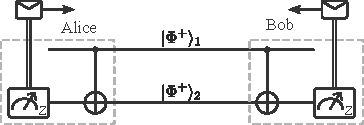
\includegraphics[width=0.7\textwidth]{lesson12/12-4_purification.pdf}
    \caption[Entanglement purification for Pauli X errors]{Entanglement purification for detecting Pauli $X$ errors.}
    \label{fig:12-4_purificaiton}
\end{figure}
Let's now introduce the detailed protocol for entanglement purification for the Pauli $X$ error, pictured in Fig.~\ref{fig:12-4_purificaiton}.
The horizontal wires represent Bell pairs shared between Alice and Bob.
Ideally, these states are $\ket{\Phi^+}_1$ and  $\ket{\Phi^+}_2$, but due to noise they will be mixed states $\rho_1$ and $\rho_2$.
Alice applies a CNOT gate on the qubits in her possession.
Qubit from the first pair acts as the control and qubit from the second pair is the target.
Bob also performs a CNOT gate on his two qubits.
Alice and Bob then measure the qubits of the second pair in Pauli $Z$ basis and send the measurement outcomes to each other using a classical message.
They keep the first pair if the measurement outcomes are the same, meaning they both measured the state \ket{0} or they both measured the state \ket{1}.
Otherwise they discard the first pair, as different measurement outcomes signal that an error has been detected.

Why this particular sequence of steps works will become more clear when we write them out mathematically.
We start by considering the ideal case where Alice and Bob share two copies of \ket{\Phi^+}.
We label the two qubits that are sent to Alice as $A_1$ and $A_2$, while Bob's qubits are $B_1$ and $B_2$.
Expanding the initial state and applying the CNOT gates,
\begin{align}
    |\Phi^{+}\rangle_{1} |\Phi^{+}\rangle_{2} & = (|00\rangle + |11\rangle)_{A_1B_1} (|00\rangle + |11\rangle)_{A_2B_2} \nonumber\\
    & = |00\rangle |00\rangle + |00\rangle |11\rangle + |11\rangle |00\rangle +|11\rangle |11\rangle \nonumber\\
    & \stackrel{\mathrm{CNOT}_{A}}{\longrightarrow} |00\rangle|00\rangle+|00\rangle|11\rangle+|11\rangle|10\rangle+|11\rangle|01\rangle \\
    & \stackrel{\mathrm{CNOT}_{B}}{\longrightarrow} |00\rangle|00\rangle+|00\rangle|11\rangle+|11\rangle|00\rangle+|11\rangle|11\rangle \nonumber \\
    & = |\Phi^{+}\rangle_{1} |\Phi^{+}\rangle_{2} \nonumber.
    \label{eq:12-4_purification_ideal}
\end{align}
In the above, we have omitted the normalization constants for clarity.
We see that the CNOT gates have left our initial state unaffected.
Measuring the second pair in Pauli $Z$ basis will give us the state \ket{00} with probability $1/2$, or the state \ket{11} with probability of $1/2$.
The outcomes will always be correlated and therefore Alice and Bob will always keep the first pair.
As well as they should since the first pair is not affected by an error.

Let's see what happens when the first pair is affected by a Pauli $X$ error.
Repeating the same calculation as in Eq.~(\ref{eq:12-4_purification_ideal}), we get
\begin{align}
    |\Psi^{+}\rangle_{1} |\Phi^{+}\rangle_{2} & = (|01\rangle + |10\rangle)_{A_1B_1} (|00\rangle + |11\rangle)_{A_2B_2} \nonumber\\
    & = |01\rangle |00\rangle + |01\rangle |11\rangle + |10\rangle |00\rangle +|10\rangle |11\rangle \nonumber\\
    & \stackrel{\mathrm{CNOT}_{A}}{\longrightarrow} |01\rangle|00\rangle+|01\rangle|11\rangle + |10\rangle|10\rangle+|10\rangle|01\rangle \\
    & \stackrel{\mathrm{CNOT}_{B}}{\longrightarrow} |01\rangle|01\rangle+|01\rangle|10\rangle+|10\rangle|10\rangle+|10\rangle|01\rangle \nonumber \\
    & = |\Psi^{+}\rangle_{1} |\Psi^{+}\rangle_{2} \nonumber.
    \label{eq:12-4_purification_error}
\end{align}
This time the error from the first pair has propagated onto the second pair.
Measuring the second pair now yields either \ket{01} or \ket{10}, both with equal probability of $1/2$.
Since the measurement outcomes are anti-correlated, Alice and Bob discard the first pair.

Now we are in a position where we can consider both initially distributed pairs to be in the mixed state given by Eq.~(\ref{eq:12-4_bitflip_mixed_state}),
\begin{equation}
    \rho_1 \otimes \rho_2 = \left[ F |\Phi^+\rangle \langle\Phi^+| + (1 - F) |\Psi^+\rangle \langle\Psi^+| \right]_1 \otimes \left[ F |\Phi^+\rangle \langle\Phi^+| + (1 - F) |\Psi^+\rangle \langle\Psi^+| \right]_2.
\end{equation}
We have already covered the situation where both Bell pairs are unaffected by noise, which occurs with probability of $F^2$, and where the first pair is bit-flipped, occurring with probability of $(1-F)F$.
The remaining two possibilities of only the second pair being bit-flipped, and both pairs being bit-flipped can be calculated in exactly same way.
We summarize all 4 possibilities in the Table.
\begin{table}[t]
    \centering
    \begin{tabular}{|l|l|l|l|l|l|l|}
        \hline Pair 1 & Pair 2 & Prob. & Meas. result & Agree? & Action & Result \\
        \hline$\left|\Phi^{+}\right\rangle$ & $\left|\Phi^{+}\right\rangle$ & $F^{2}$ & 00 or 11 & Y & Keep & $\left|\Phi^{+}\right\rangle$ \\
        \hline$\left|\Phi^{+}\right\rangle$ & $\left|\Psi^{+}\right\rangle$ & $F(1-F)$ & 01 or 10 & N & Discard & N/A \\
        \hline$\left|\Psi^{+}\right\rangle$ & $\left|\Phi^{+}\right\rangle$ & $(1-F) F$ & 01 or 10 & N & Discard & N/A \\
        \hline$\left|\Psi^{+}\right\rangle$ & $\left|\Psi^{+}\right\rangle$ & $(1-F)^{2}$ & 00 or 11 & Y & Keep & $\left|\Psi^{+}\right\rangle$ \\
        \hline
    \end{tabular}
    \caption[X error purification]{Purification for Pauli $X$ error.}
    \label{tab:12-4_purification_X_error}
\end{table}
We can make an interesting observation.
When both initial pairs are affected by the Pauli $X$ error, the purification procedure still tells Alice and Bob to keep the first pair, because the measurement outcomes on the second pair are correlated.
This occurs with probability $(1-F)^2$ and is the ``false positive'' that we mentioned earlier in this Section.

The total success probability of this purification procedure is
\begin{equation}
    \text{Pr} \{\text{success}\} = F^2 + (1 - F)^2.
\end{equation}
The state that Alice and Bob share after a successful purification is
\begin{equation}
    \rho = F' |\Phi^+\rangle\langle\Phi^+| + (1 - F') |\Psi^+\rangle\langle\Psi^+|,
\end{equation}
where the new fidelity $F'$ is related to the initial one via
\begin{align}
    F^{\prime}=\frac{F^{2}}{F^{2}+(1-F)^{2}}.
\end{align}
The expression for the new post-purification fidelity is very interesting.
When $F > 0.5$, the fidelity of the purified state increases, $F' > F$.
The name for the process, purification, is now more clear.
We start with a noisy state and end up with a new state of higher quality, a more pure state.

% This is just a simple example of purification, and does not cover all of the operational details.
% You can learn more from advanced materials, such as research papers, Professor Van Meter's first book, or future modules that we will be creating.



\section{Making a network}

% Step Five: Making a Network

So far, we have considered how to create entanglement between neighboring nodes, so link-level entanglement, how to extend this with entanglement swapping to end-to-end entanglement, so entanglement between nodes that are not physically connected directly. Now let's consider what it takes to actually create a network. There are a few problems, but the two main problems that we will consider in this step are routing (how you direct traffic through a network), and also multiplexing and resource management.

Let's say that we have some complicated network like this, and we wish to communicate from this point over here, all the way down to this point over there. The job of a network is to establish a connection between those two nodes. In quantum networks, we wish to establish an entangled pair between those two nodes such that we can either use it for some quantum key distribution, or for teleportation, or for any other purposes we may wish to consider. So how does the network know how to do it? Well, it has to first content with the first problem, that's routing.

How does it pick a particular path where it performs entanglement swapping? Well, let's consider a simpler case of the following network- so let's say that we want to communicate from A to E. We can see that there are three different possible paths that the network can take. It can establish an entangled pair between A and E by performing entanglement swapping at B, or it can do it by entanglement swapping between D while it's sharing link-level entanglement between D-E and A-E, or it can go via the node C and perform entanglement swapping there, as well as D. So first it needs to establish link-level entanglement between A-D, D-C, C-E, and then perform entanglement swapping on the qubits at C and entanglement swapping on the qubits at D in order to establish end-to-end entanglement between A and E.

What we need in order to evaluate which way is best, is to look at the cost that it takes to establish link-level entanglement, and then how to combine these costs in order to establish the cost for the entire path, so for the entire end-to-end entanglement. So one possible way of evaluating the link-level entanglement is to evaluate the cost of establishing a link-level entanglement- is seconds per bell pairs at a threshold fidelity. So what does that mean? As we said, in order to establish entanglement, let's say between A and B, we have to first make the quantum memories that are sitting at A emit a photon, and quantum memory sitting at $B$ to emit a photon, and then they have to meet, let's say in the middle, if we are considering the memory interference- memory setup where the photons can be measured in a Bell state basis, and that will entangle the memories at A and at B, but these photons will get lost in the fiber- they will get attenuated. So this procedure is not deterministic. Sometimes we get lucky and the link-level entanglement can be established quickly. Sometimes we have to wait a little bit longer. So the more lossy the channel is, the more lossy the fiber is, the more we are expected to wait a little bit longer for the Bell pairs to get established. And in order to make this comparison fair, we set a fixed fidelity, that we are looking to establish bell pairs at a given fidelity, and this is usually dictated by the protocol that we want to run, or for by the end-to-end distance between the nodes A and E. So this gives us a good idea for a cost of establishing the link-level entanglement. Now, how do we combine these costs for each individual links in order to know the full cost of establishing end-to-end entanglement over a longer path? Well, one possibility is to use Dijkstra's shortest path first algorithm. So what we can do is we can sum the costs for the path A-B-E in order to obtain a good estimate of the full total cost of establishing end-to-end entanglement, or we can do it for A-D-E and A-D-C-E. This way the network can know what's actually best, and it will be able to deliver the entire end-to-end entanglement more efficiently. And by knowing which path is most efficient, of course it knows how to route information and establish an end-to-end entanglement.

So the next problem that we have to deal with is multiplexing, and that can be demonstrated by considering the following scenario- we have a bunch of nodes over here that are all connected to a node E, and here on the right side again, we have the following tree that's leading to node F. So let's say that A is trying to communicate with K. Well, we can use link-level entanglement between E-F, F-K, and A-E, and then apply entanglement swapping at E, entanglement swapping at F, in order to obtain end-to-end entanglement between A-K. But what if different two nodes also are trying to communicate? Let's say that $B$ wants to establish end-to-end entanglement with node J. They have to go through the link E-F. This creates contention on E-F link, so the network needs to know how to handle such requests where a single link has to be shared between two different pairs- between pair A-K and B-J.

Furthermore, we can have more network nodes trying to establish end-to-end entanglement. This case, we can have C-H, C and H, or we can even have the case where we have node G trying to communicate with node K, and this creates contention on the following link, on the link F-I, that the network needs to know how to handle such requests.

In this chapter, we have seen the four requirements for building a quantum network. So first we started at the bottom with a basic building block, and that's how to establish entanglement between two neighboring nodes of a network, meaning establishing link-level entanglement and how to handle photon losses. Next, we saw how we can establish end-to-end entanglement, meaning entanglement between nodes which don't share a direct physical link using entanglement swapping. Then we talked about how to handle errors, how to improve the quality of our distributed state, and namely we introduced the protocol of purification, and finally in this last step we gave you a little bit more idea what it takes to build the network that there are other considerations that we have to take into account, such as routing, multiplexing and resource management. But this is all just building a single network. Quantum Internet is a different beast entirely. Quantum Internet is a network of quantum networks, so that we will discuss in the coming chapters.


\newpage
\begin{exercises}
\exer{Consider the following quantum state:}
\begin{equation*}
\ket{\psi} = \frac{\sqrt{3}}{2}\ket{0} + \frac{1}{2}\ket{1}
\end{equation*}
\subexer{Find the probability of measuring a zero.}
\subexer{Find the probability of measuring a one.}


\end{exercises}

